\documentclass[compress]{beamer}

\usepackage[nofonts]{ctex}
\setCJKmainfont[ItalicFont={Kaiti SC}]{Kaiti SC}%
%\setCJKmainfont[ItalicFont={AR PL KaitiM GB}]{AR PL KaitiM GB}%
%\setCJKsansfont{WenQuanYi Zen Hei}% 文泉驿的黑体


\mode<beamer>
{
    \setbeamercovered{transparent}
    \useinnertheme{rounded}
    \useoutertheme{split}
    \usecolortheme{rose}
    \usecolortheme{seahorse}

	\expandafter\def\expandafter\insertshorttitle\expandafter{%
	\insertshorttitle\hfill%
	\insertframenumber\,/\,\inserttotalframenumber}
}

\mode<handout>
{
	\usetheme{default}
	\usepackage{pgfpages}
	\pgfpagesuselayout{4 on 1}[a4paper,landscape,border shrink=5mm]
}


\usepackage{amsmath,latexsym,amssymb,amsfonts,amsbsy}
\usepackage{graphicx}
\usepackage{hyperref}
\usepackage{listings}
\usepackage{fancyvrb}
\fvset{frame=single,fontsize=\scriptsize}

\newcommand{\romannumber}[1]{{\textrm{\uppercase\expandafter{\romannumeral
#1}}}}
\setbeamercolor{dblue}{fg=white,bg=blue!40!black} % for beamercolorbox
\newenvironment{pblock}{\begin{beamercolorbox}[rounded=true,
          shadow=true]{dblue}}{\end{beamercolorbox}}


\graphicspath{{figure/}}

\lstset{
	basicstyle=\ttfamily\footnotesize, % print whole listing footnotesize
	keywordstyle=\ttfamily\color{black}\bfseries, 
	identifierstyle=\ttfamily\color{blue}, 
	commentstyle=\ttfamily\itshape, 
	stringstyle=\ttfamily,
	frame=single, 
	numbers=left, numberstyle=\tiny,
	stepnumber=1, numbersep=10pt,
	showtabs=false, tabsize=4,
	showstringspaces=false,
	breaklines=true, breakatwhitespace=true,
	language=[ISO]C++
}   

%%%%%%%%%%%%%%%%%%%%%%%%%%%%%%%%%%%%%%%%%%%%%%%%%%%%%%%%%%%%%%%%%
%    body                                                       %
%%%%%%%%%%%%%%%%%%%%%%%%%%%%%%%%%%%%%%%%%%%%%%%%%%%%%%%%%%%%%%%%%


\begin{document}

\AtBeginSection[]
{ 
    \begin{frame}<beamer> 
		\frametitle{内容提要} 
		\tableofcontents[currentsection,currentsubsection] 
	\end{frame} 
} 
					
\title{文档制作}

\author[\href{http://c.pku.edu.cn/}{http://c.pku.edu.cn/}]
{曹东刚\\\href{mailto:caodg@sei.pku.edu.cn}{caodg@sei.pku.edu.cn}}

\institute{Linux程序设计环境 \\
\href{http://c.pku.edu.cn/}{
http://c.pku.edu.cn/}}

\date{}

\titlegraphic{\includegraphics[height=0.17\textwidth]{Overlays/logo.pdf}}

\begin{frame}
	\titlepage
\end{frame}

\section{排版系统}

\begin{frame}
\frametitle{版面设计}
\begin{itemize}
\item 版面设计是一门艺术. 文档的可理解性和可读性非常重要
    \begin{itemize}
      \item 结构清晰: 标题序号与字体大小要适当
      \item 页面美观: 行宽适当
    \end{itemize}

\item 作者、图书设计者、排版者
    \begin{itemize}
      \item 作者: 交付图书原稿给出版公司
      \item 图书设计者: 决定整本书的版面形式(栏宽、字体、行距、标题前后间距等), 给出排版说明
      \item 排版者: 根据排版说明进行排版
    \end{itemize}

\end{itemize}

\end{frame}

\begin{frame}
\frametitle{电子排版系统}

\begin{itemize}
\item 所见即所得(WYSIWYG)的文字处理软件
    \begin{itemize}
    \item M\$ Word, WPS, Open Office, Word Perfect, 等等
    \end{itemize}
\item 格式化排版程序
    \begin{itemize}
    \item 首先编辑一个文本的源文件
        \begin{itemize}
          \item 文档正文部分(作者)
          \item 文档结构描述部分(图书设计者)
        \end{itemize}
    \item 然后用排版程序对源文件进行格式化处理(排版者)
    \item 将结果输出到输出设备, 如监视器或打印机等
    \end{itemize}
\end{itemize}


\end{frame}

\begin{frame}
  \frametitle{Unix排版系统}
  \begin{itemize}
    \item troff, groff
	\item texinfo
	\item \TeX{}与\LaTeX
	\item docbook
	\item 轻量标记语言: asciidoc, Markdown, reStructedText
  \end{itemize}
  
\end{frame}

\section{\LaTeX}

\begin{frame}
\frametitle{\LaTeX{}排版的公式}
\small
\begin{align}
\begin{split}
|I_1| &= \left| \int_\Omega gRu \,d\Omega \right| \\
&\le C_3 \left[ \int_\Omega \left( \int_{a}^x
g(\xi,t) \,d \xi \right)^2d \Omega \right]^{1/2} \\
&\quad\times \left[ \int_\Omega \left\{ u^2_x + \frac{1}{k}
\left( \int_{a}^x cu_t \, d\xi \right)^2 \right\}
c \Omega \right]^{1/2} \\
&\le C_4 \left| \left| f \left| \widetilde{S}^{-1,0}_{a,-}
W_2(\Omega,\Gamma_l) \right| \right|
\left| |u| \overset{\circ} \to W_2^{\widetilde{A}}
(\Omega;\Gamma_r,T) \right| \right|.
\end{split}\label{eq:A} \\
\begin{split}
|I_2| &= \left| \int_{0}^T \psi(t) \left\{ u(a,t)
-\int_{\gamma(t)}^a \frac{d\theta}{k(\theta,t)}
\int_{a}^\theta c(\xi) u_t(\xi,t) \,d \xi \right\} dt
\right| \\
&\le C_6 \left| \left| f \int_\Omega
\left| \widetilde{S}^{-1,0}_{a,-}
W_2(\Omega,\Gamma_l) \right| \right|
\left| |u| \overset{\circ} \to W_2^{\widetilde{A}}
(\Omega;\Gamma_r,T) \right| \right|.
\end{split}
\end{align}

\end{frame}

\begin{frame}
\frametitle{\TeX{}与Donald E. Knuth}
Stanford大学的计算机科学家 Donald E. Knuth (高德纳) 在上世纪70年代设计了\TeX{}和Metafont

\begin{minipage}{0.4\hsize}
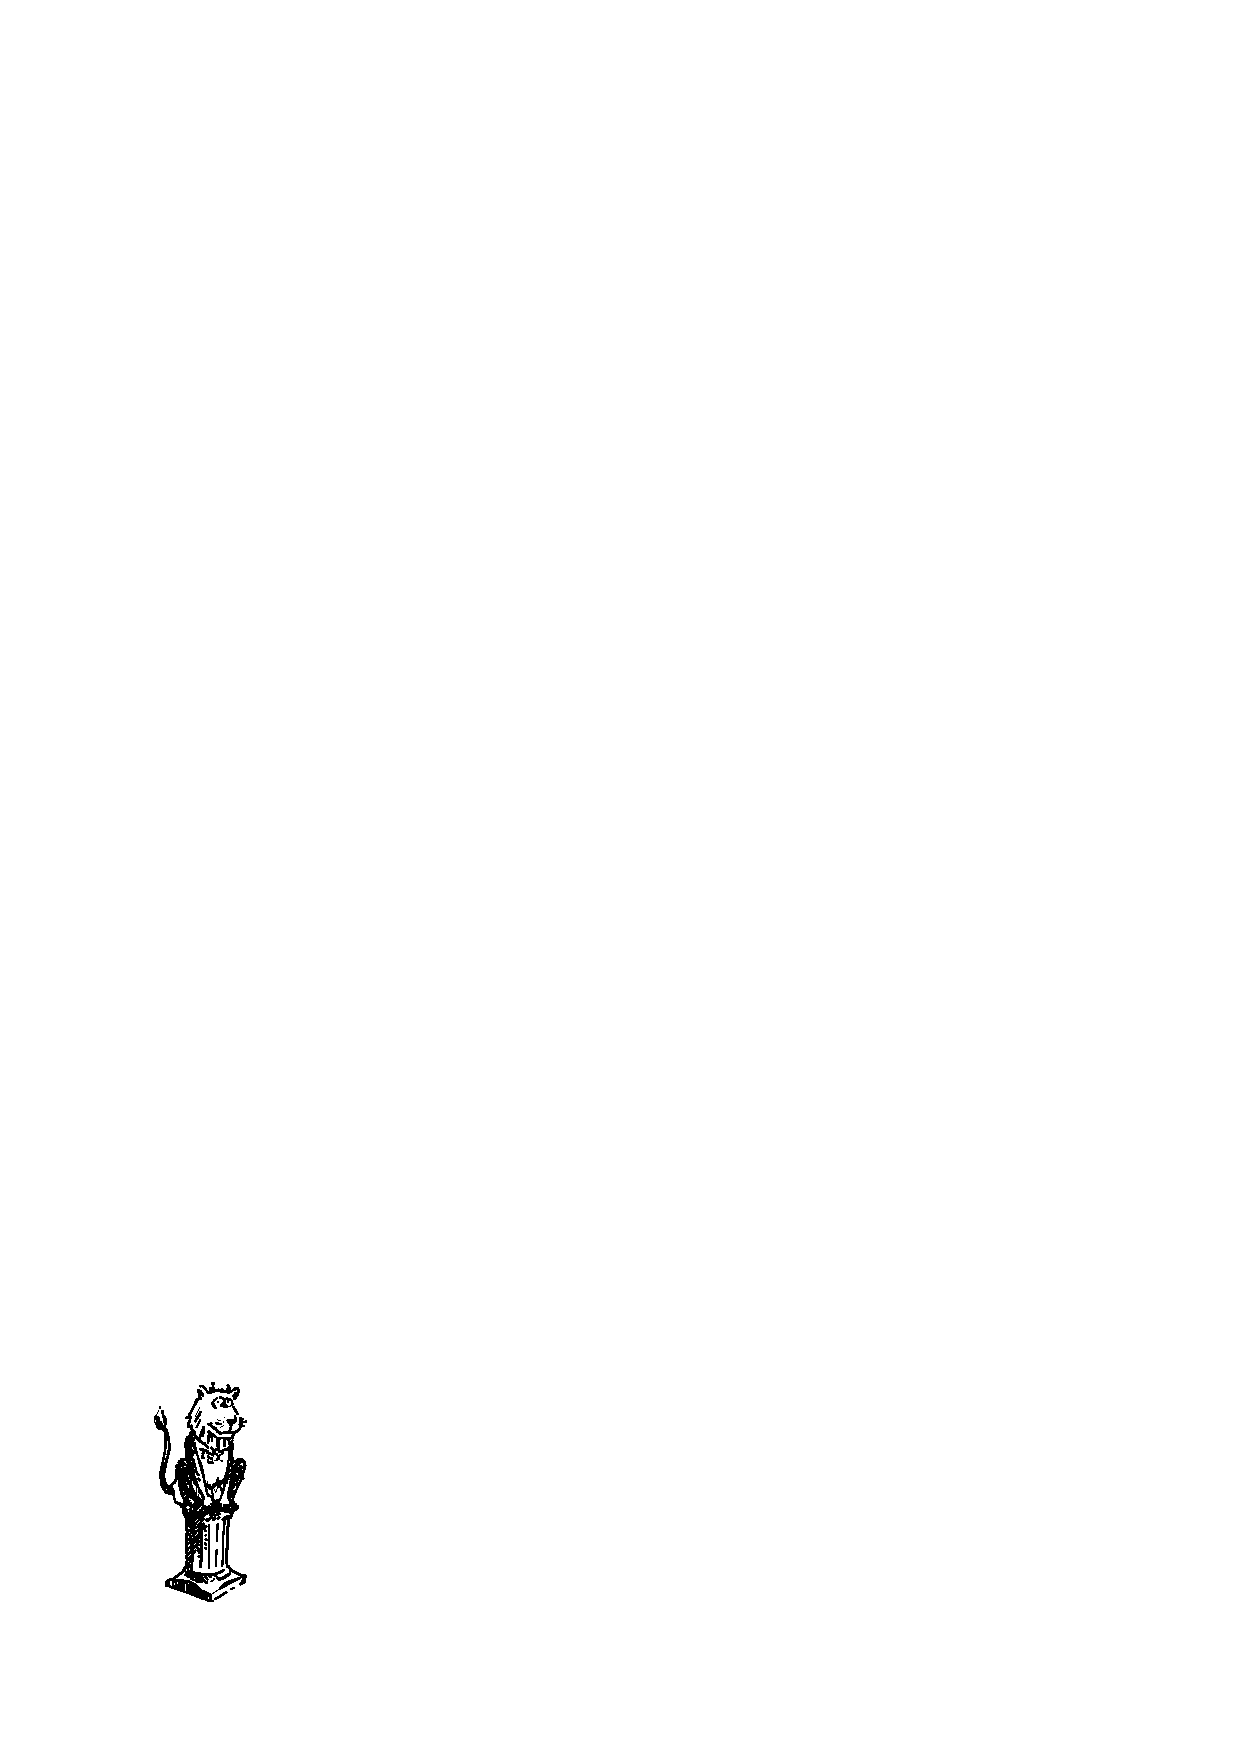
\includegraphics[width=0.9\hsize]{tex.pdf}\\
\centering \TeX
\end{minipage}\hfill%
\begin{minipage}{0.4\hsize}

\includegraphics[width=0.9\hsize]{meta.pdf}\\
\centering Metafont
\end{minipage}

\end{frame}

\begin{frame}
\frametitle{\TeX{}历史与现状}

\begin{itemize}
\item 1978: \TeX{}第一版面世, 用Pascal书写, 输出与设备无关
\item 1982: \TeX{}稳定版本, 自此之后极少修订
\item 1993: Knuth 宣布冻结\TeX{}与Metafont, 不再进行更新
\item 1995至今: 只发现一个\TeX{}的排版错误, 非软件错误

\end{itemize}
\TeX{}与Metafont最新版本:
\begin{itemize}
\item \TeX{}版本: 3.141592, 收敛到\emph{$\pi$}
\item Metafont版本: 2.718, 收敛到\emph{$e$}
\end{itemize}
\end{frame}


\begin{frame}
\frametitle{\TeX{}扩展}
最基本的 \TeX 程序只是由一些很原始的命令组成, 难于使用
\begin{itemize}
\item Plain \TeX: Knuth 设计了一个名叫 Plain \TeX 的基本格式
    \begin{itemize}
      \item Plain \TeX 的重点还只是关注于如何排版
    \end{itemize}
\item AMS \TeX{}与 AMS \LaTeX: 美国数学协会提供的, 基于Plain \TeX
    \begin{itemize}
    \item 用于排版含有很多数学符号和公式的科技类文章或书籍
    \end{itemize}
\item \LaTeX: Leslie Lamport 1985年开发, 最流行和使用最为广泛
    \begin{itemize}
      \item 构筑在 Plain \TeX 的基础之上, 并加进了很多的功能
      \item 基本上不需要使用者自己设计命令和宏等, 易学易用
      \item \LaTeX{}2.09, \LaTeX{}3, \LaTeXe
    \end{itemize}

\end{itemize}
\end{frame}


\begin{frame}
\frametitle{\TeX{}/\LaTeX{}的不足}

\begin{itemize}
\item 不适合没有灵魂、没有思想的人\footnote{``\LaTeX does not work well for people who have sold their souls \ldots''}

\item 不能马上完全学会, 除非你是一个天才

\item 即使开端良好, 也难以掌握其精髓

\item 当发生错误的时候, 对新手而言排错可能是很困难的

\item 设计一个新的版面非常困难

\item 不适合排版非结构化的、无序的文档
\end{itemize}


\end{frame}

\begin{frame}
\frametitle{\TeX{}/\LaTeX{}的优势}

\begin{itemize}

\item 高质量、专业级的输出
\item 记住几个说明文档逻辑结构的命令即可应付多数情况
\item 适合具有良好结构的文档
\item 可很容易地生成目录、索引、脚注、引用等复杂结构
\item 是可编程的, 易于定制与扩展
\item \TeX{}引擎是免费、开源的, 具有超常的稳定性
\item 良好的通用性与跨平台性
\item 超级技术支持, 众多的免费资源
\item 一种乐趣
\end{itemize}

\end{frame}



\begin{frame}
\frametitle{接受\LaTeX{}的出版社}
几乎所有的世界一流学术出版机构, 包括
\begin{itemize}
\item AMS
\item Elsevier
\item Kluwer Academic Publishers
\item Cambridge University Press
\item Springer
\item IEEE
\item \ldots
\end{itemize}
\end{frame}

\begin{frame}
\frametitle{\TeX{}的未来}

下面列出了几个正在进行中的对\TeX{}进行扩展的项目:

\begin{itemize}
\item PDFTeX : 完全兼容标准的 \TeX , 但能够给出 PDF 输出
\item e-\TeX : 不仅完全兼容标准的 \TeX , 还支持一种``扩展模式''
\item Omega : 几乎是完全重新写过的、支持 Unicode 的 \TeX 程序
\item NTS : NTS 代表``New Typesetting System'', 将来可能取代\TeX{}或e-\TeX
\item XeTeX: 内置Unicode支持的\LaTeX
\item LuaTeX: 基于PDFTeX, 以Lua为嵌入式脚本语言,目标是增加开放和扩展性
\end{itemize}

\end{frame}


\begin{frame}
\frametitle{\LaTeX{} vs Word}
\begin{itemize}
\item 易用: Word (所见即所得)
\item 稳定美观: \LaTeX
\item 办公文档: Word
\item 科技论文: \LaTeX
\item 短文: Word
\item 复杂结构的长文档: \LaTeX
\end{itemize}

\end{frame}

\begin{frame}
  \frametitle{\LaTeX{}学习要点}
\begin{itemize}
\item 找一本详尽的使用手册, 通读所有内容, 了解\LaTeX 的全部功能, 但不必记住所有
的命令
\item 尽早使用各种高级功能, 如定理环境、公式、索引、交叉引用等
\item 尽量选取最恰当的命令实现所需要的功能
\item 尽量复用成熟的格式文件, 如各种科技论文宏包, 学位论文宏包等
\item 选择一个或几个好的画图工具
\end{itemize}

\end{frame}


\begin{frame}
\frametitle{\LaTeX{}系统}
\begin{itemize}
\item web2c: C语言实现的\TeX{}系统, GPL版权保护
    \begin{itemize}
      \item 很多重要的free \LaTeX{}实现都基于web2c
    \end{itemize}
\item teTeX: 基于web2c, 大多数Unix/Linux系统的缺省安装
\item web2c-win32: 即ftTeX, web2c 的 Win32 实现
\item MikTeX: Windows下最好用的\LaTeX{}实现, 更新很快
\item Tex Live: \href{http://tug.org/texlive/}{http://tug.org/texlive/},
    主流发行版
    \begin{itemize}
    \item 基于teTeX与web2c-win32, 支持 Unix/Linux/Mac OS/Windows
    \end{itemize}
\item CTeX与ChinaTeX: 集成MikTeX, 增加中文支持(CCT与CJK)
\end{itemize}

\end{frame}

\begin{frame}
\frametitle{中文支持}
\begin{itemize}
\item CCT: 由中科院计算所张林波等设计
    \begin{itemize}
     \item 在文档格式方面相当符合中文习惯
     \item 与\LaTeX{}的辅助程序兼容性较差
     \item 最新版本的CCT兼容性有很大提高
    \end{itemize}
\item CJK: 由欧洲人(Werner Lemberg) 设计
    \begin{itemize}
    \item 与\LaTeX 的辅助程序兼容性相当好
    \item 在文档格式方面的中文化较差
    \item 逐渐成为中文处理的主流
    \end{itemize}
\end{itemize}

\end{frame}

\begin{frame}
\frametitle{\LaTeX{}文档处理步骤}

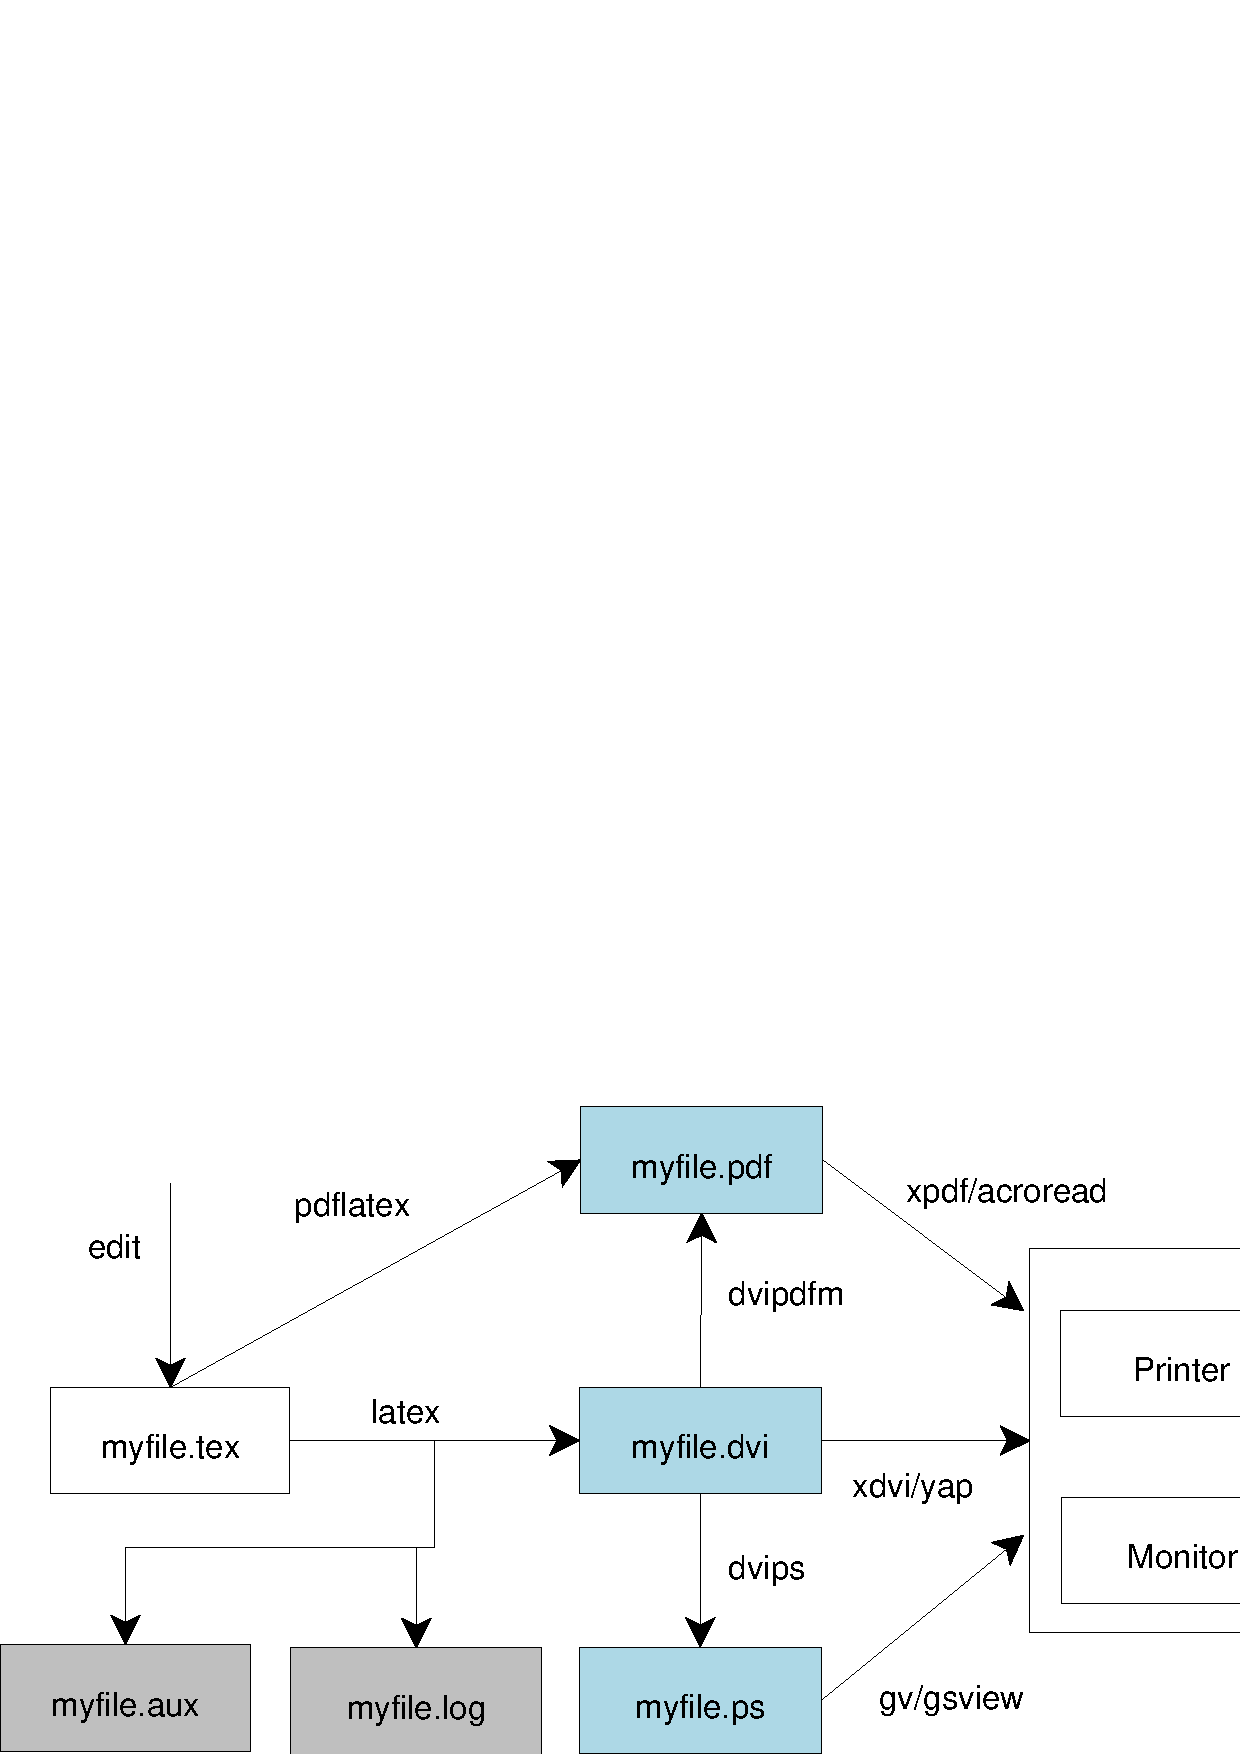
\includegraphics[width=\hsize]{latexprocess.pdf}
\end{frame}

\begin{frame}[containsverbatim]
\frametitle{各类常见\LaTeX{}文件}
\begin{tabular}{p{1cm}p{10cm}}\hline
.tex & \TeX{}或\LaTeX{}源文件, 可用latex处理 \\
.sty & \LaTeX{}宏包文件, 可用\verb~\usepackage~加载 \\
.dtx & 文档化的\LaTeX{}文件, \LaTeX{}宏包发布的主要格式 \\
.ins & 相应的.dtx文件的安装文件. 可用latex对.ins文件处理, 从.dtx中提取出宏包 \\
\hline
.dvi & 设备无关文件, 可预览排版效果 \\
.log & 记录编译的详细信息 \\
.toc & 记录所有章节的标题, 第二次编译时读入生成目录 \\
.aux & 记录交叉引用等信息, 用于向第二次编译传递信息 \\
.idx & 记录所有的索引词条, 需用makeindex生成\\
.lof & 记录所有的图形目录\\

\end{tabular}

\end{frame}


\begin{frame}[containsverbatim]
\frametitle{PS文件与PDF文件}
\begin{itemize}
\item 从tex文件生成pdf文件: \verb"caodg@debian:~$ pdflatex myfile.tex"
\item 从dvi文件生成ps文件: \verb"caodg@debian:~$ dvips myfile"
\item 从ps文件生成pdf文件: \verb"caodg@debian:~$ ps2pdf myfile.ps"
\item 查看ps文件: \verb"caodg@debian:~$ gv myfile.ps"
\item 查看pdf文件: \verb"caodg@debian:~$ xpdf myfile.ps"
\end{itemize}
查看ps文件与pdf文件的工具有多种

\end{frame}

\begin{frame}
    \frametitle{\LaTeX{}编辑工具}
  \begin{itemize}
	\item vim + latexsuite
	\item emacs
	\item lyx (WYSIWYG)
	\item WinEdt (commercial)
  \end{itemize}
  
\end{frame}


\begin{frame}[containsverbatim]
\frametitle{\LaTeX{}源文件}
为普通的ASCII文件, 包含待排版的文本和如何排版的命令
\begin{itemize}
\item 空白距离: 空格、制表符等空白字符被视为相同的空白距离\\
多个连续空白字符等同于一个空白字符\\
空行标志段落结束; 多个连续空行等同一个空行
\item 特殊字符: \verb[# $ % ^ & _ { } ~ \[ \\
除\verb~\~外, 上述其它字符皆可通过前面加反斜杠得到
\item 命令: 大小写敏感, 以反斜杠开始加上只包含字母字符命令名\\
如, \verb~ \TeX \emph{emphasize} \today ~
\item 注释: 百分号\verb~%~后面的字符、分行符、下一行开始的空白字符全部视为注释
\end{itemize}

\end{frame}

\begin{frame}
\frametitle{文档和语言的结构}
文档的主旨在于向读者传递观点、信息和知识, 如果排版风格反映了内容的逻辑和语义结构,
读者就会抓住文章脉络.\\

\LaTeX{}只需要你告诉它文档的逻辑和语义结构
\begin{itemize}
\item 段落: \LaTeX{}中最重要的文档单位
\item 句子: \LaTeX{}中较小的文档单位
    \begin{itemize}
      \item 句子也有结构, 谨慎使用标点符号
    \end{itemize}
\item 逻辑结构: 章、节、子节等高级结构
\end{itemize}


\end{frame}

\begin{frame}[containsverbatim]
\frametitle{最简单的\LaTeX{}源文件}

\begin{Verbatim}
\documentclass{article}
\begin{document}
Hello world!
\end{document}
\end{Verbatim}


\end{frame}

\begin{frame}[containsverbatim]
\frametitle{\LaTeX{}源文件结构}
\begin{Verbatim}
\documentclass[选项]{文档类}
\usepackage[options]{package}
全局命令与定义
\begin{document}
文本与局部命令
\end{document}
\end{Verbatim}

\begin{itemize}
\item 导言(preamble): \verb~\begin{document}~之前的内容, 对宏包的引用放在导言区
\item 正文(body): \verb~\begin{document}~之后的内容
\end{itemize}

\end{frame}

\begin{frame}[containsverbatim]
\frametitle{文档类}
\LaTeX{}处理源文件时, 首先需要知道要处理的文档类型, 例\\
\verb~\documentclass[11pt,twoside,a4paper]{article}~\\

文档类:
\begin{itemize}
\item article : 排版科技文章、短报告、程序文档等
\item report : 排版多章的长报告、短篇书籍、博士论文等
\item book : 排版书籍
\item frames : 排版幻灯片
\end{itemize}


\end{frame}

\begin{frame}
\frametitle{文档类选项}
\begin{itemize}
\item 10pt(缺省), 11pt, 12pt
\item a4paper, b5paper, letterpaper(缺省)
\item fleqn : 数学公式左对齐, 而不是中间对齐
\item leqno : 公式编号居左
\item titlepage, notitlepage : 文档标题后是否分页
\item onecolumn, twocolumn : 单列或双列排版
\item twoside, oneside : 双面或单面格式
\item openright, openany : 新章在奇数页开始还是下一页开始
\end{itemize}

\end{frame}


\begin{frame}[containsverbatim]
\frametitle{篇章结构示例}


\begin{Verbatim}
\documentclass[a4paper,11pt]{article}
\usepackage{amsmath}
\title{Demonstrate \LaTeX Structure}
\author{Donggang Cao}
\begin{document}
% generates the title
\maketitle
% insert the table of contents
\tableofcontents
\section{Begin}
Well, and here begins my lovely article.
\subsection{Theorem One}
\section{Conclusion}
Here it ends.
\end{document}
\end{Verbatim}

\end{frame}

\begin{frame}
\begin{tabular}{|l|}\hline
\includegraphics[width=0.5\hsize]{struct.pdf}\\
\hline
\end{tabular}
\end{frame}

\begin{frame}[containsverbatim]
\frametitle{大型文档}
处理大型文档如书籍、博士论文时, 最好将源文件分为几个部分
\begin{itemize}
\item 方法1: include和includeonly命令\\
    在正文区: \verb~\include{filename}~, 在新页开始排版\\
    在导言区: \verb~\includeonly{filename}~\\
    只有includeonly声明的文件会被包含进来, 可用于大型文档的草稿调试阶段
\item 方法2: \verb~\input{filename}~命令, 在当前位置排版\\
    既可在正文区, 也可在导言区, 常用于包含设置文件等
\end{itemize}


\end{frame}

\begin{frame}[containsverbatim]
\frametitle{环境}
一个环境用命令\verb~\begin{环境}~开始, 以\verb~\end{环境}~结束\\
环境的作用在于: 其内的文本要根据环境参数进行不同的处理,  有可能暂时
改变处理特征, 如行距、字体、缩进等. 这些改变只在环境内起作用\\
常见的环境
\begin{itemize}
\item itemize, enumerate, description
\item flushleft, flushright, center
\item quote, quotation, verse
\item verb, verbatim
\end{itemize}
\end{frame}

\begin{frame}[containsverbatim]
\frametitle{列表环境}

\begin{Verbatim}
\begin{enumerate}
\item You can mix the list environments to your taste:
\begin{itemize}
\item But it might start to look silly.
\item[-] With a dash.
\end{itemize}
\item Therefore remember:
\begin{description}
\item[Stupid] things will not become smart because they are in a list.
\item[Smart] things, though, can be presented beautifully in a list.
\end{description}
\end{enumerate}
\end{Verbatim}


\end{frame}

\begin{frame}
\frametitle{列表环境输出}

\begin{enumerate}
\item You can mix the list
environments to your taste:
\begin{itemize}
\item But it might start to
look silly.
\item[-] With a dash.
\end{itemize}
\item Therefore remember:
\begin{description}
\item[Stupid] things will not
become smart because they are
in a list.
\item[Smart] things, though, can be
presented beautifully in a list.
\end{description}
\end{enumerate}

\end{frame}


\begin{frame}[containsverbatim]
\frametitle{数学公式}
文档结构是\LaTeX{}的灵魂; 数学是\TeX{}的灵魂\\
\LaTeX{}用数学模式来排版数学符号和公式, 以区分通常的文本模式
\begin{itemize}
\item 数学模式中的空格和分行都被忽略. 空格要么是公式的逻辑衍生物, 要么通过命令得到
\item 数学模式不允许有空行, 每个公式中只能有一个段落
\item 每个字符都被看作变量名进行排版. 如果要插入文本, 需要用命令输入
\end{itemize}
如果希望在当前行排版数学公式, 可用\verb~$公式内容$~界定

\end{frame}

\begin{frame}[containsverbatim]
\frametitle{公式示例}

\begin{Verbatim}
\begin{displaymath}
\lim_{n \to \infty}
\sum_{k=1}^n \frac{1}{k^2}
= \frac{\pi^2}{6}
\end{displaymath}
\end{Verbatim}
输出结果:
\begin{displaymath}
\lim_{n \to \infty}
\sum_{k=1}^n \frac{1}{k^2}
= \frac{\pi^2}{6}
\end{displaymath}

\end{frame}

\begin{frame}[containsverbatim]
\frametitle{图形}
\LaTeX{}可以直接生成简单的图形, 包括文本、各种斜率的直线、箭头、矩形、椭圆形等\\
图形环境\\[1ex]

\begin{tabular}{|l|}\hline
\begin{minipage}{0.9\hsize}
\vspace{2mm}
\renewcommand{\baselinestretch}{1.3}
\begin{verbatim}

\begin{picture}(x尺寸, y尺寸)
画图命令
\end{picture}
\end{verbatim}
\vspace{1mm}
\end{minipage}\\
\hline
\end{tabular}


\end{frame}

\begin{frame}[containsverbatim]
\frametitle{图形示例}

\begin{Verbatim}
\setlength{\unitlength}{2cm}
\begin{picture}(5,2)\thicklines
  \put(5,0){\vector(-1,0){5}}
  \put(0,0){\vector(1,1){2}}
  \put(2,2){\vector(3,-2){3}}
\end{picture}
\end{Verbatim}
\begin{minipage}{0.6\hsize}
\setlength{\unitlength}{2cm}
\begin{picture}(5,2)\thicklines
  \put(5,0){\vector(-1,0){5}}
  \put(0,0){\vector(1,1){2}}
  \put(2,2){\vector(3,-2){3}}
\end{picture}
\end{minipage}
\end{frame}


\begin{frame}
\begin{minipage}[b]{0.9\hsize}
\setlength{\unitlength}{0.2in}
\begin{picture}(15,15)\thicklines
  \put(5,0){\line(1,0){5}}
  \put(5,0){\line(2,1){10}}
  \put(5,0){\line(1,1){10}}
  \put(5,0){\line(1,3){5}}
  \put(5,0){\line(0,1){15}}
  \put(5,0){\line(-1,2){5}}
  \put(5,0){\line(-1,1){5}}

  \put(10,0){\line(1,1){5}}
  \put(10,0){\line(1,2){5}}
  \put(10,0){\line(0,1){15}}
  \put(10,0){\line(-1,3){5}}
  \put(10,0){\line(-1,1){10}}
  \put(10,0){\line(-2,1){10}}

  \put(15,5){\line(0,1){5}}
  \put(15,5){\line(-1,2){5}}
  \put(15,5){\line(-1,1){10}}
  \put(15,5){\line(-3,1){15}}
  \put(15,5){\line(-1,0){15}}

  \put(15,10){\line(-1,1){5}}
  \put(15,10){\line(-2,1){10}}
  \put(15,10){\line(-3,0){15}}
  \put(15,10){\line(-3,-1){15}}

  \put(10,15){\line(-1,0){5}}
  \put(10,15){\line(-2,-1){10}}
  \put(10,15){\line(-1,-1){10}}

  \put(5,15){\line(-1,-1){5}}
  \put(5,15){\line(-1,-2){5}}

  \put(0,10){\line(0,-1){5}}
\end{picture}
\end{minipage}

\end{frame}

\begin{frame}[containsverbatim]
\frametitle{正文内的引用}
\begin{itemize}
  \item 交叉引用\\
  首先标记: \verb~\label{chap01:sec1:fig:myfig}~
  引用: \verb~\ref{chap01:sec1:fig:myfig}~
  \item 参考文献的引用\\
  首先生成参考文献\\
  引用: \verb~\cite[附加信息]{关键词}~

\end{itemize}

\end{frame}

\begin{frame}[containsverbatim]
\frametitle{生成参考文献}

\noindent 最好的方法是通过参考文献数据库生成, 运行命令\alert{bibtex}

\begin{itemize}
\item 首先, 声明样式\verb~\bibliographystyle{样式}~\\
   常用样式
   \begin{itemize}
     \item plain : 文献按字母顺序排列
     \item unsrt : 文献按\verb~\cite~命令出现的先后排列
   \end{itemize}

\item 然后, 引用文献数据库\verb~\bibliography{数据库文件}~\\
   数据库文件在计算机上以.bib为扩展名, 此处只给出主干名
\end{itemize}

\end{frame}

\begin{frame}[containsverbatim]
\frametitle{文献数据库}

参考文献数据库条目示例:\\[1ex]

\begin{Verbatim}
@book{Haters94,
  author        = "Simson Garfinkel and Daniel Weise",
  title         = "The UNIX-HATERS Handbook",
  publisher     = "IDG Books",
  address       = "California",
  year          = "1994",
  url           = "http://www.simson.net/ref/ugh.pdf"
};
\end{Verbatim}
\end{frame}

\begin{frame}
\frametitle{用\LaTeX{}制作幻灯}
  推荐工具
  \begin{itemize}
	\item beamer
	\item pdfscreen + ppower4
	\item foiltex
	\item prosper
	\item texpower
  \end{itemize}
  
\end{frame}


\section{绘图}


\begin{frame}
\frametitle{\LaTeX{}插图}

\begin{itemize}
\item 当~Knuth~编写~\TeX~的时候,还没有~PostScript/EPS, JPEG, GIF~等, 因此~DVI~并不直接支持这些格式的图形.
不过,\TeX{}允许~DVI~文件中包含~\alert{special}~命令来向~DVI~处理程序传递命令

\item 1994~年发布的~\LaTeXe{}~的图形宏包套件增加了对图形的支持

\item 由于~DVI~文件经常被转为~PS~文件,所以支持最好的是对~EPS~格式~(Encapsulated %
Post\-Script, 是~PS~语言的子集)~的图像

\end{itemize}
\end{frame}


\begin{frame}
\frametitle{xfig}
\alert{xfig}是功能非常强大的画矢量图的工具, 可以方便的导出为各种图形格式. 缺点在于绘图习惯大多数人不适应\\
\href{http://www.xfig.org}{http://www.xfig.org}

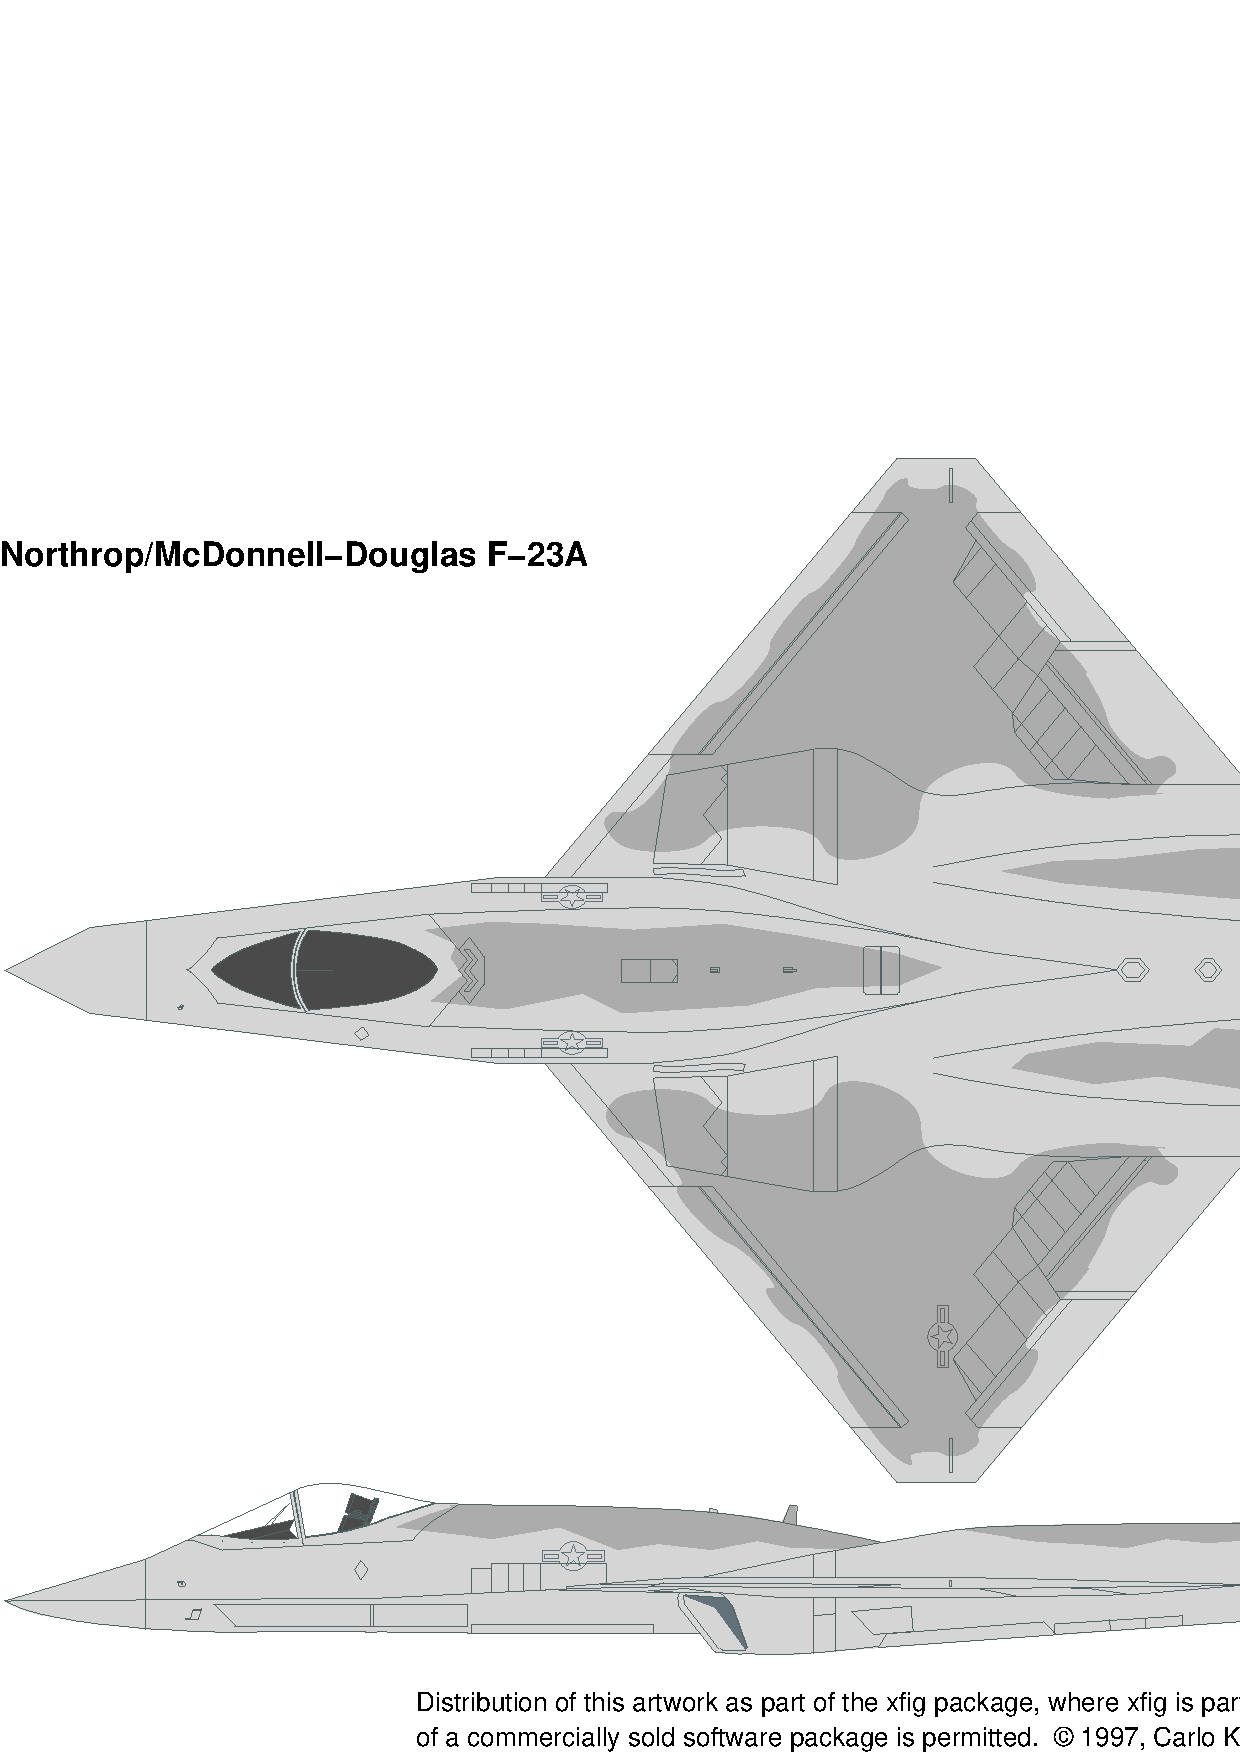
\includegraphics[width=0.6\hsize]{plane.pdf}


\end{frame}

\begin{frame}
\frametitle{dia}
\alert{dia}是基于GTK的绘图工具, 类似于windows下的\alert{visio}\\
\href{http://www.gnome.org/projects/dia/}{http://www.gnome.org/projects/dia/}

\includegraphics[width=0.6\hsize]{dia_screen.jpg}
\end{frame}

\begin{frame}
\frametitle{Gnuplot}
\alert{gnuplot}是将数据和函数转换为专业的图表的工具, 可以实现比M\$ excel强大的多的绘图功能\\
\href{http://www.gnuplot.info/}{http://www.gnuplot.info/}

\includegraphics[width=0.5\hsize]{title2.png}%
\includegraphics[width=0.5\hsize]{surface.png}
\end{frame}


\begin{frame}
\frametitle{MetaPost}
MetaPost~是基于~Knuth~的~Metafont~的绘图语言, 可以产生 PostScript 输出. 唯一的缺点就是太强大、太精确了\\
\href{http://www.tug.org/metapost.html}{http://www.tug.org/metapost.html}

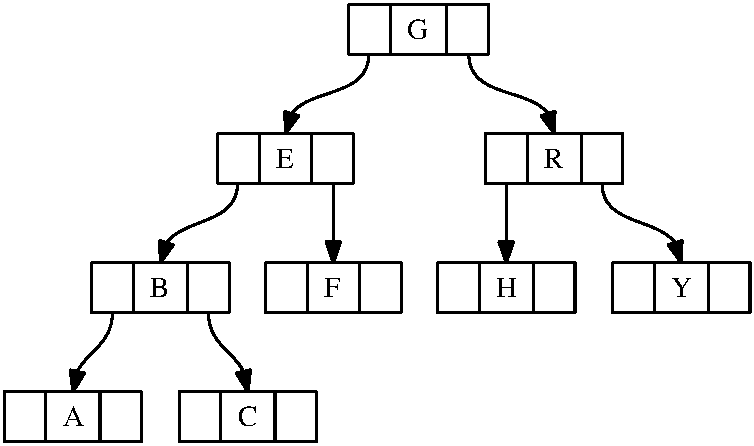
\includegraphics[width=0.4\hsize]{tree.png}%
\includegraphics[width=0.6\hsize]{ex4.png}

\end{frame}

\begin{frame}
	\frametitle{graphviz}
	Graphviz (Graph Visualization Software的缩写)是一个由AT\&T实验室启动的开源工具包,用于绘制DOT语言脚本描述的图形。Graphviz是一个自由软件,其授权为Common Public License。
\end{frame}

\begin{frame}
	\frametitle{graphviz构架}
Graphviz由一种被称为DOT语言的图形描述语言与一组可以生成和/或处理DOT文件的工具组成:

\begin{itemize}
	\item dot : 一个用来将生成的图形转换成多种输出格式的命令行工具。其输出格式包括PostScript,PDF,SVG,PNG,含注解的文本等等。
	\item neato : 用于sprint model的生成。
	\item twopi : 用于放射状图形的生成。
	\item circo : 用于圆形图形的生成。
	\item fdp : 另一个用于生成无向图的工具。
	\item dotty : 一个用于可视化与修改图形的图形用户界面程序。
	\item lefty : 一个可编程的控件,可以显示DOT图形。
\end{itemize}
	
\end{frame}

\begin{frame}[containsverbatim]
	\frametitle{graphviz示例: Hello World}

\begin{Verbatim}
echo "digraph G {Hello->World}" | dot -Tpng >hello.png 
\end{Verbatim}

\centering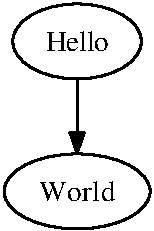
\includegraphics[width=0.3\hsize]{helloworld.pdf}
	
\end{frame}

\begin{frame}[containsverbatim]
	\frametitle{graphviz示例: 数据结构-树}
\centering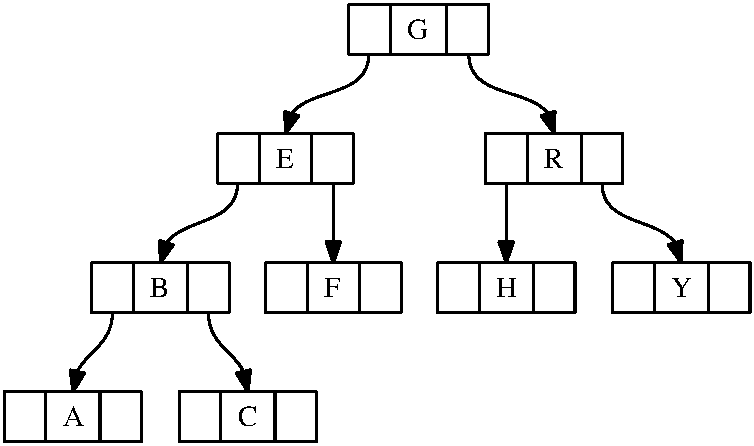
\includegraphics[width=0.9\hsize]{tree.pdf}
\end{frame}

\begin{frame}[containsverbatim]
	\frametitle{graphviz示例: 数据结构-树}
	{\tiny
\begin{verbatim}
digraph g {  
    node [shape = record,height=.1];  
    node0[label = "<f0> |<f1> G|<f2> "];  
    node1[label = "<f0> |<f1> E|<f2> "];  
    node2[label = "<f0> |<f1> B|<f2> "];  
    node3[label = "<f0> |<f1> F|<f2> "];  
    node4[label = "<f0> |<f1> R|<f2> "];  
    node5[label = "<f0> |<f1> H|<f2> "];  
    node6[label = "<f0> |<f1> Y|<f2> "];  
    node7[label = "<f0> |<f1> A|<f2> "];  
    node8[label = "<f0> |<f1> C|<f2> "];  
    "node0":f2 -> "node4":f1;  
    "node0":f0 -> "node1":f1;  
    "node1":f0 -> "node2":f1;  
    "node1":f2 -> "node3":f1;  
    "node2":f2 -> "node8":f1;  
    "node2":f0 -> "node7":f1;  
    "node4":f2 -> "node6":f1;  
    "node4":f0 -> "node5":f1;  
    } 
\end{verbatim}
}
\end{frame}

\begin{frame}
    \frametitle{在\LaTeX{}直接绘图: Tikz}
    \noindent 示例见:
    \href{http://www.texample.net/tikz/examples/}{http://www.texample.net/tikz/examples/}
\centering\includegraphics[width=0.9\hsize]{3d-cone.pdf}
\end{frame}

\begin{frame}
    \frametitle{在\LaTeX{}直接绘图: Tikz}
\centering\includegraphics[width=0.6\hsize]{dandelin-spheres.pdf}
\end{frame}

\begin{frame}
    \frametitle{在\LaTeX{}直接绘图: Tikz}
\centering\includegraphics[width=0.7\hsize]{christmas-tree-2.pdf}
\end{frame}

\begin{frame}
    \frametitle{在\LaTeX{}直接绘图: Tikz}
\centering\includegraphics[width=0.9\hsize]{merge-sort-recursion-tree.pdf}
\end{frame}

\section{Docbook}

\begin{frame}
  Docbook是一种基于XML的新式文档工具
  \begin{itemize}
	\item 很多开源软件的标准文档工具
	\item 文档结构DTD和样式单
	\item 各种XML处理工具的支持
	\item 适合项目文档, 不适合学术报告
  \end{itemize}
  
\end{frame}

\section{程序文档}

\begin{frame}
	\frametitle{Doxygen}
doxygen是一个自动文档生成系统,它对使用C++, C, Java, Objective-C, Python, IDL, PHP, C\#等语言编写的代码及注释进行分析,自动生成说明文档。Doxygen支持多种格式的说明文档,包括html, RTF(Word), Latex, XML等。 
\end{frame}

\begin{frame}
	\frametitle{DoxygenToolkit.vim}
	VIM插件,自动生成
	\begin{itemize}
		\item License 模板: DoxLic
		\item Author 模板: DoxAu
		\item 注释模板: Dox
	\end{itemize}
\end{frame}

\begin{frame}[containsverbatim]
	\frametitle{Doxygen示例}
	{ \tiny
\begin{verbatim}
/* Copyright (C)
 * BSD blablabla...
 */

/**
 * @file A.java
 * @brief bababa
 * @author Donggang Cao
 * @version 1.0
 * @date 2011-05-15
 */

public class A {
    /**
     * @brief main : blabla
     *
     * @param args : blabla
     *
     * @return : blabla
     */
    public static void main(String[] args) { }
}
\end{verbatim}
}
\end{frame}

\section{幻灯片}
\begin{frame}
    \frametitle{幻灯片制作}
    \begin{block}{传统工具}
            PowerPoint, Keynote, Beamer, Google Presentation
    \end{block}

    \begin{block}{HTML展示}
        \begin{itemize}
            \item Presi, Google Presentation
            \item S5, Slidy, Impress.js
    \end{itemize}
    \end{block}
\end{frame}

\end{document}
